\section{Evaluation · Atribución, escenarios y sensibilidad}

\begin{takeaway}
Una vez validado el modelo, se usa para responder las preguntas de negocio: \textbf{(i)} qué \% de las ventas atribuimos al marketing, \textbf{(ii)} cuánto ganaríamos reasignando presupuesto desde \textit{Performance} hacia \textit{Propios y Exterior}, y \textbf{(iii)} qué tan sensible es el resultado a pequeños errores en los $\beta$.
\end{takeaway}

\subsection{Calidad del ajuste recap}

\begin{figure}[htbp]
\centering
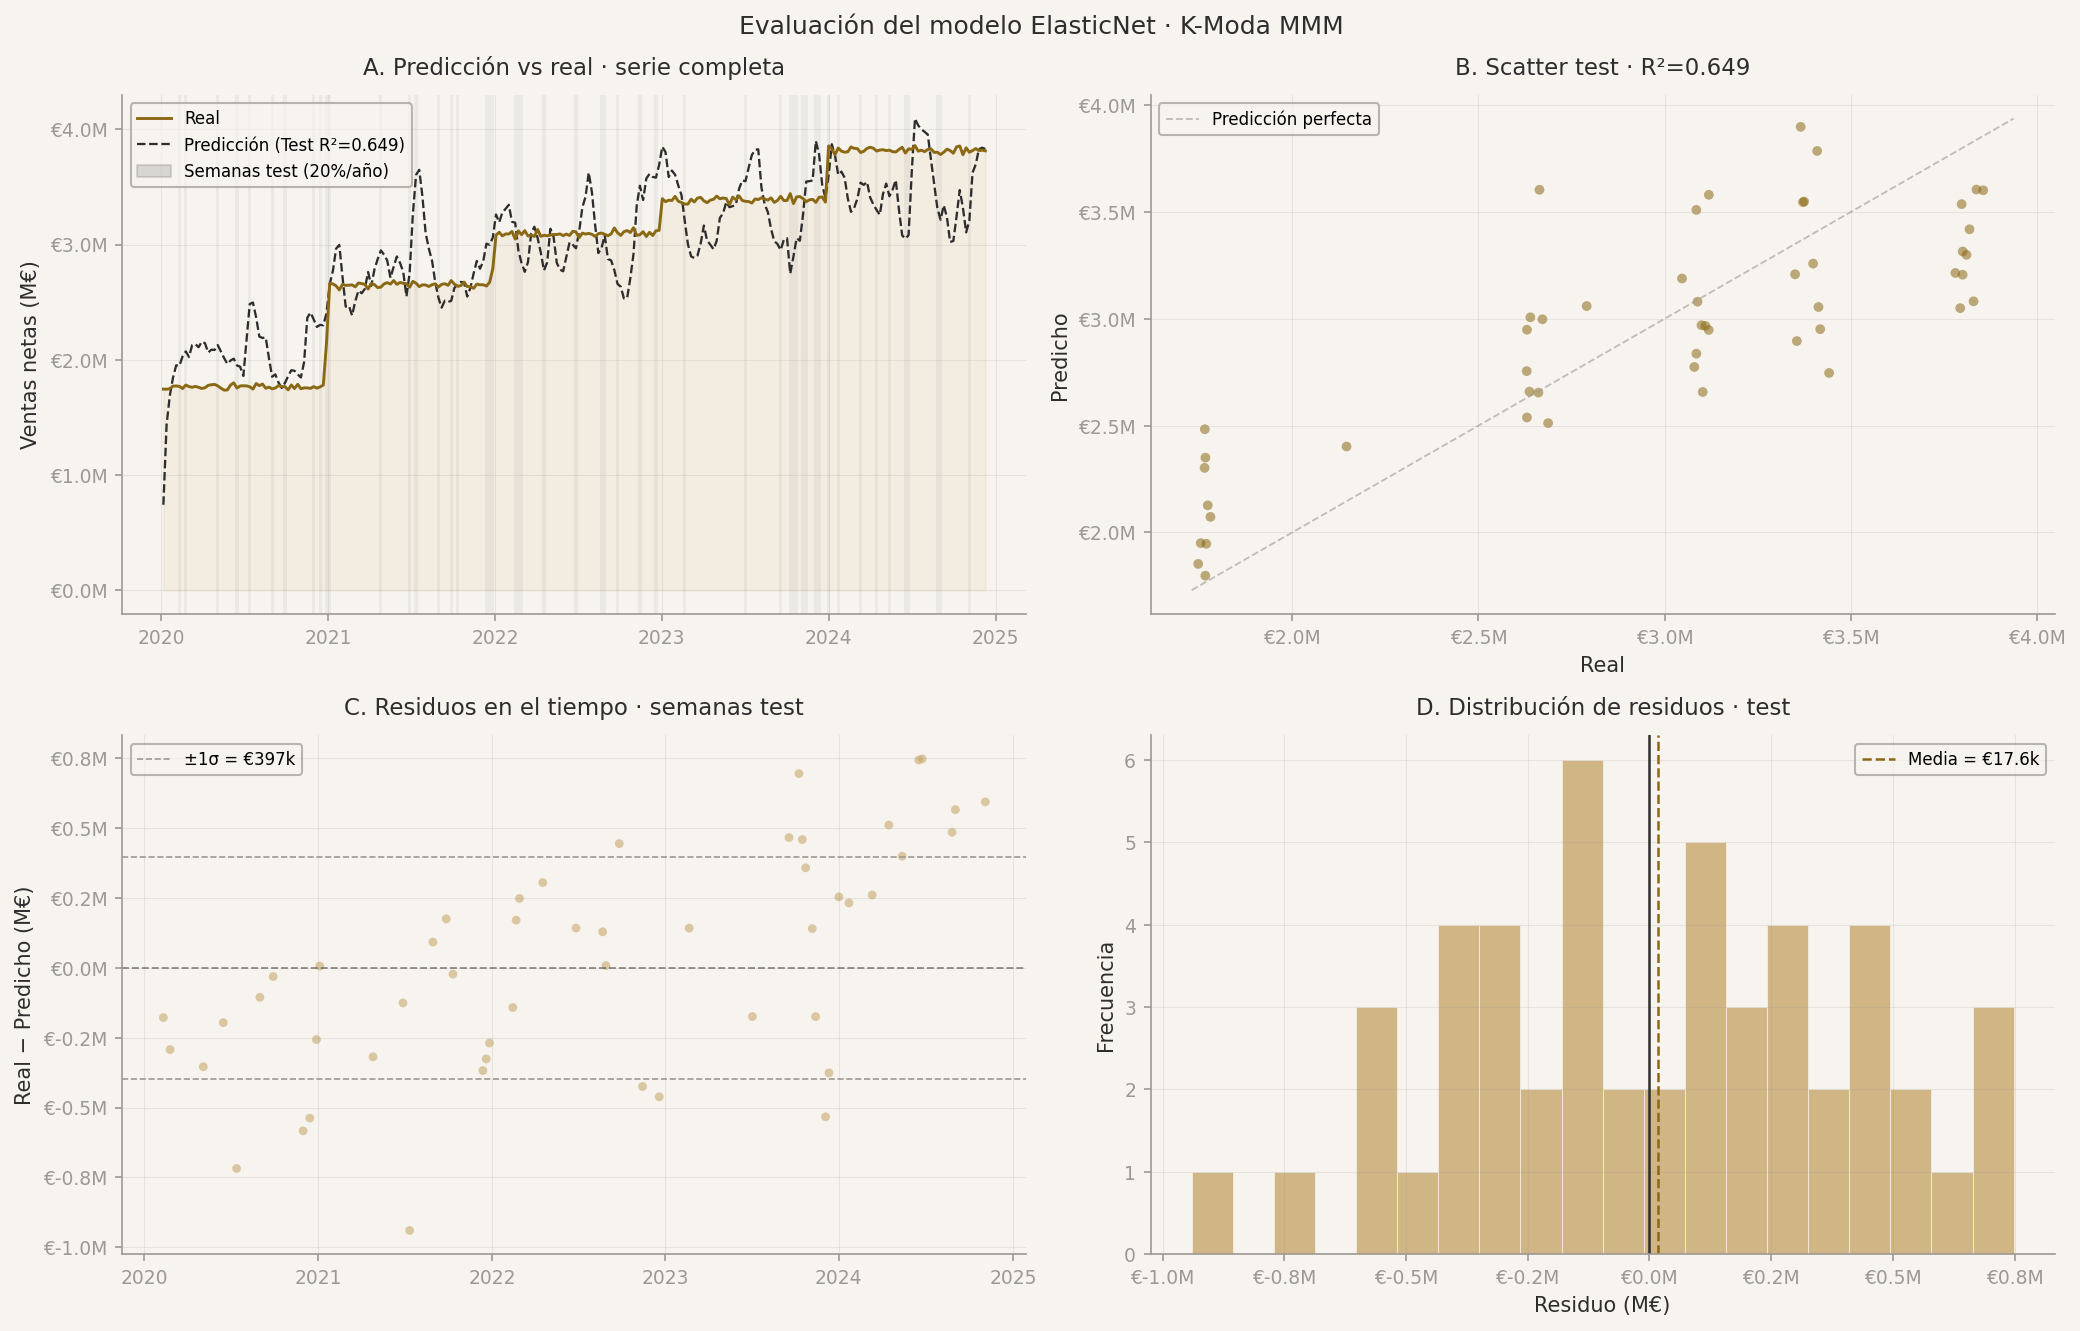
\includegraphics[width=\textwidth]{figures/ev_g1_ajuste.png}
\caption{\textbf{Ajuste del modelo revisitado.} Línea real vs. predicción, con separación visual entre train y test.}
\label{fig:ev_ajuste}
\end{figure}

\begin{figure}[htbp]
\centering
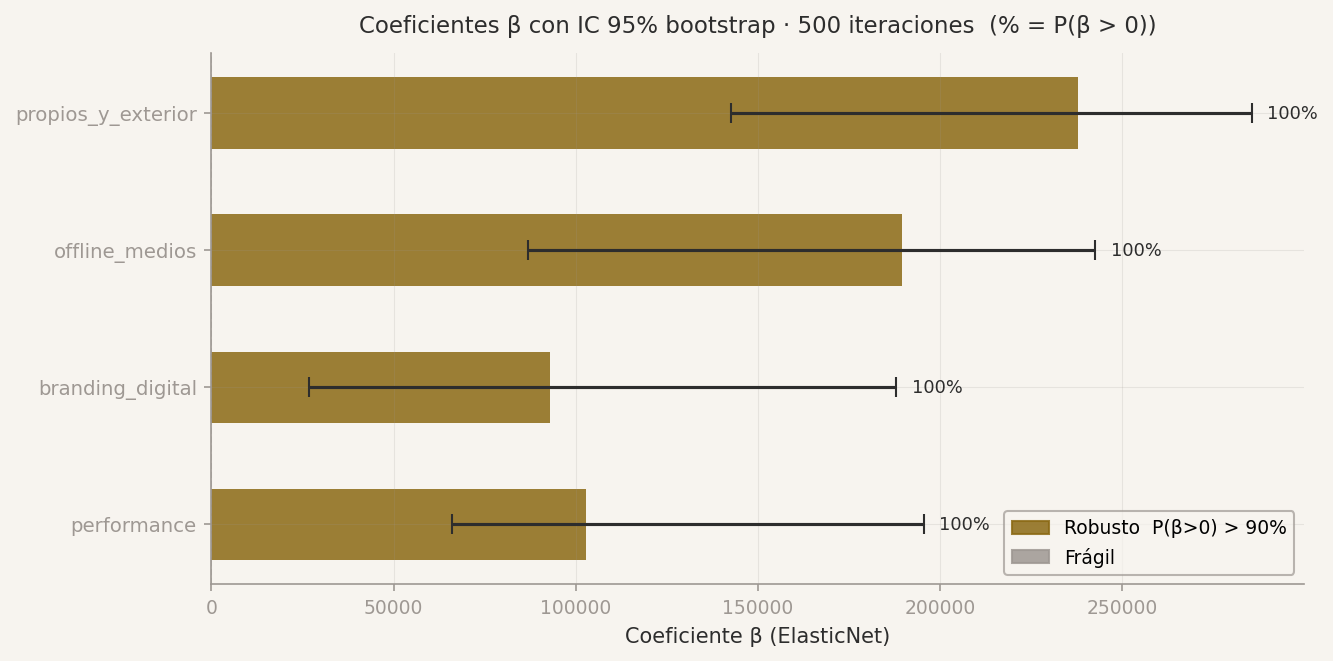
\includegraphics[width=\textwidth]{figures/ev_g2_betas.png}
\caption{\textbf{Coeficientes finales con intervalos de confianza.} Los cuatro grupos de marketing son positivos y sus IC 95\% no cruzan cero $\rightarrow$ contribución robusta.}
\label{fig:ev_betas}
\end{figure}

\subsection{Atribución · ¿Cuánto viene del marketing?}

Sobre las 258 semanas analizadas (2020--2024) y 758.1\,M€ de ventas acumuladas, la descomposición del modelo arroja:

\begin{center}
\begin{tabular}{@{}l r r r@{}}
\toprule
\textbf{Grupo} & \textbf{Inversión (M€)} & \textbf{Contribución (M€)} & \textbf{ROI} \\
\midrule
Performance            & 23.5  & 141.8 & \textbf{6.0$\times$} \\
Branding Digital       & 13.6  & 115.4 & 8.5$\times$ \\
Offline Medios         & 11.8  & 181.0 & 15.3$\times$ \\
\textbf{Propios y Exterior} & \textbf{10.0} & \textbf{256.7} & \textbf{25.7$\times$} \\
\midrule
\textbf{Total marketing}    & \textbf{58.9} & \textbf{695.0} & \textbf{11.8$\times$} (ponderado) \\
\bottomrule
\end{tabular}
\end{center}

La suma de contribuciones equivale al \textbf{91.8\% de las ventas totales} del periodo.

\begin{decisionbox}
\textbf{Nota honesta sobre el \textbf{91.8\%}.} Este número es elevado comparado con benchmarks de MMM en retail físico (típicamente 20--40\% atribuido a medios). Hay que leerlo así: es el resultado de un \textbf{contrafactual} — ``si K-Moda no hubiera invertido nada en publicidad desde 2020, el modelo predice 63\,M€ de ventas acumuladas, en lugar de los 758\,M€ observados''. Este contrafactual no contempla la \textbf{inercia de marca} que K-Moda ya tiene en 2020: parte de lo que el modelo atribuye a medios es, en realidad, memoria de campañas anteriores a 2020 que no están en los datos. El porcentaje es válido \textit{relativamente} (compara grupos entre sí) pero debe presentarse con este matiz ante el comité.
\end{decisionbox}

\begin{figure}[htbp]
\centering
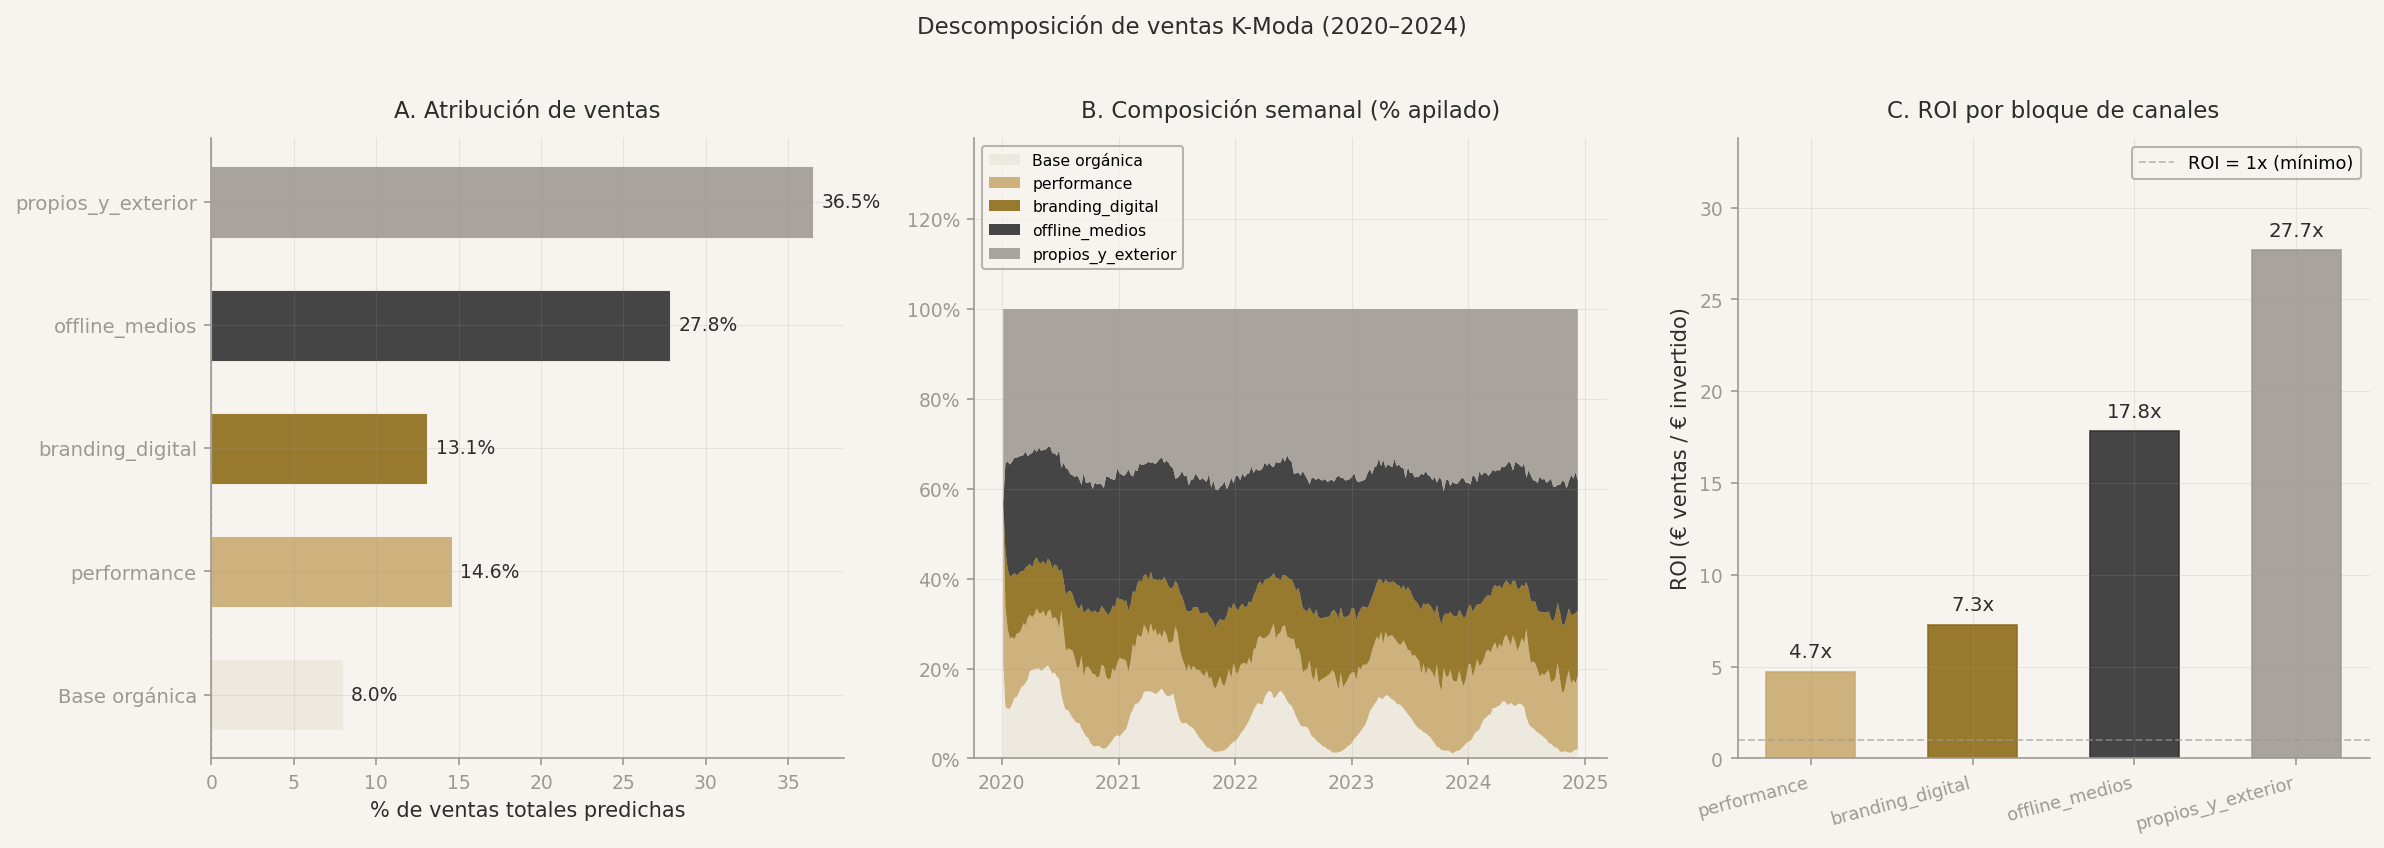
\includegraphics[width=\textwidth]{figures/ev_g3_descomposicion.png}
\caption{\textbf{Descomposición final.} Capa dorada = marketing atribuido; capa gris = base orgánica. La descomposición se lee semana a semana en el dashboard.}
\label{fig:ev_desc}
\end{figure}

\begin{decisionbox}
\textbf{Metodología de atribución (estándar MMM):}
\[
\text{Ventas predichas} = \text{Base orgánica} + \sum_{\text{grupo}} \beta_{\text{grupo}} \cdot x_{\text{grupo,escalado}}
\]
Cada grupo aporta su $\beta$ multiplicado por su variable transformada (logadstock). Sumando las cuatro contribuciones se obtiene el total atribuible; la \textit{base} es lo que quedaría con \texttt{inversión} $= 0$.
\end{decisionbox}

\subsection{Simulación de escenarios}

La función \texttt{simular(inv\_nueva)} toma un vector de inversión semanal por grupo, aplica los mismos \textit{adstocks} y saturaciones que vio el modelo, y devuelve las ventas anuales proyectadas, el \textit{lift} vs. baseline y el ROI. Con ella se definen tres escenarios canónicos:

\begin{center}
\begin{tabular}{@{}p{3.2cm} p{6.8cm} p{3.8cm}@{}}
\toprule
\textbf{Escenario} & \textbf{Descripción} & \textbf{Qué mide} \\
\midrule
\textsc{Do Nothing}    & Mantener el reparto histórico. & Baseline. \\
\textsc{Do Something}  & Transferir el 30\% del grupo con menor ROI (\textit{Performance}) al de mayor ROI (\textit{Propios y Exterior}). & Upside realista sin aumentar presupuesto. \\
\textsc{Do the Most}   & Reasignar el 60\% de Performance a Propios y Exterior. & Upside ambicioso, concentrando riesgo. \\
\bottomrule
\end{tabular}
\end{center}

\begin{figure}[htbp]
\centering
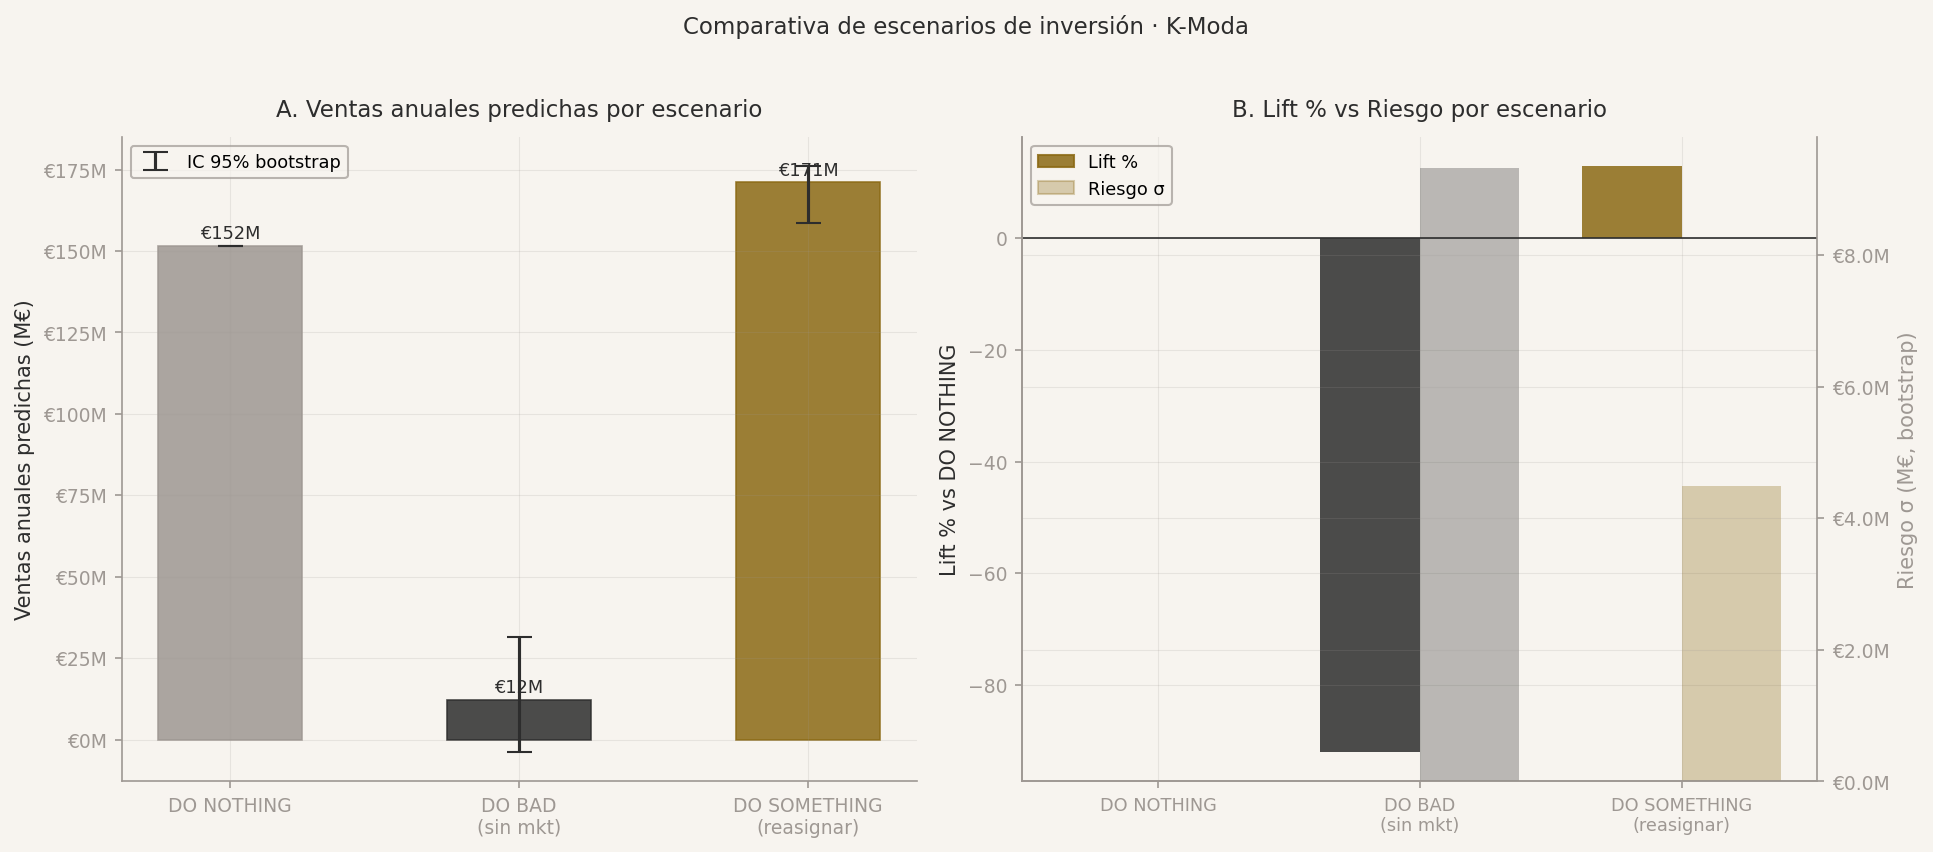
\includegraphics[width=\textwidth]{figures/ev_g4_escenarios.png}
\caption{\textbf{Comparativa de los tres escenarios.} \textsc{Do Something} captura la mayor parte del \textit{upside} con la menor perturbación al mix actual. \textsc{Do the Most} añade incremento marginal pero concentra el riesgo en un único grupo.}
\label{fig:ev_escenarios}
\end{figure}

\subsection{Curvas de respuesta · Rendimientos decrecientes}

\begin{figure}[htbp]
\centering
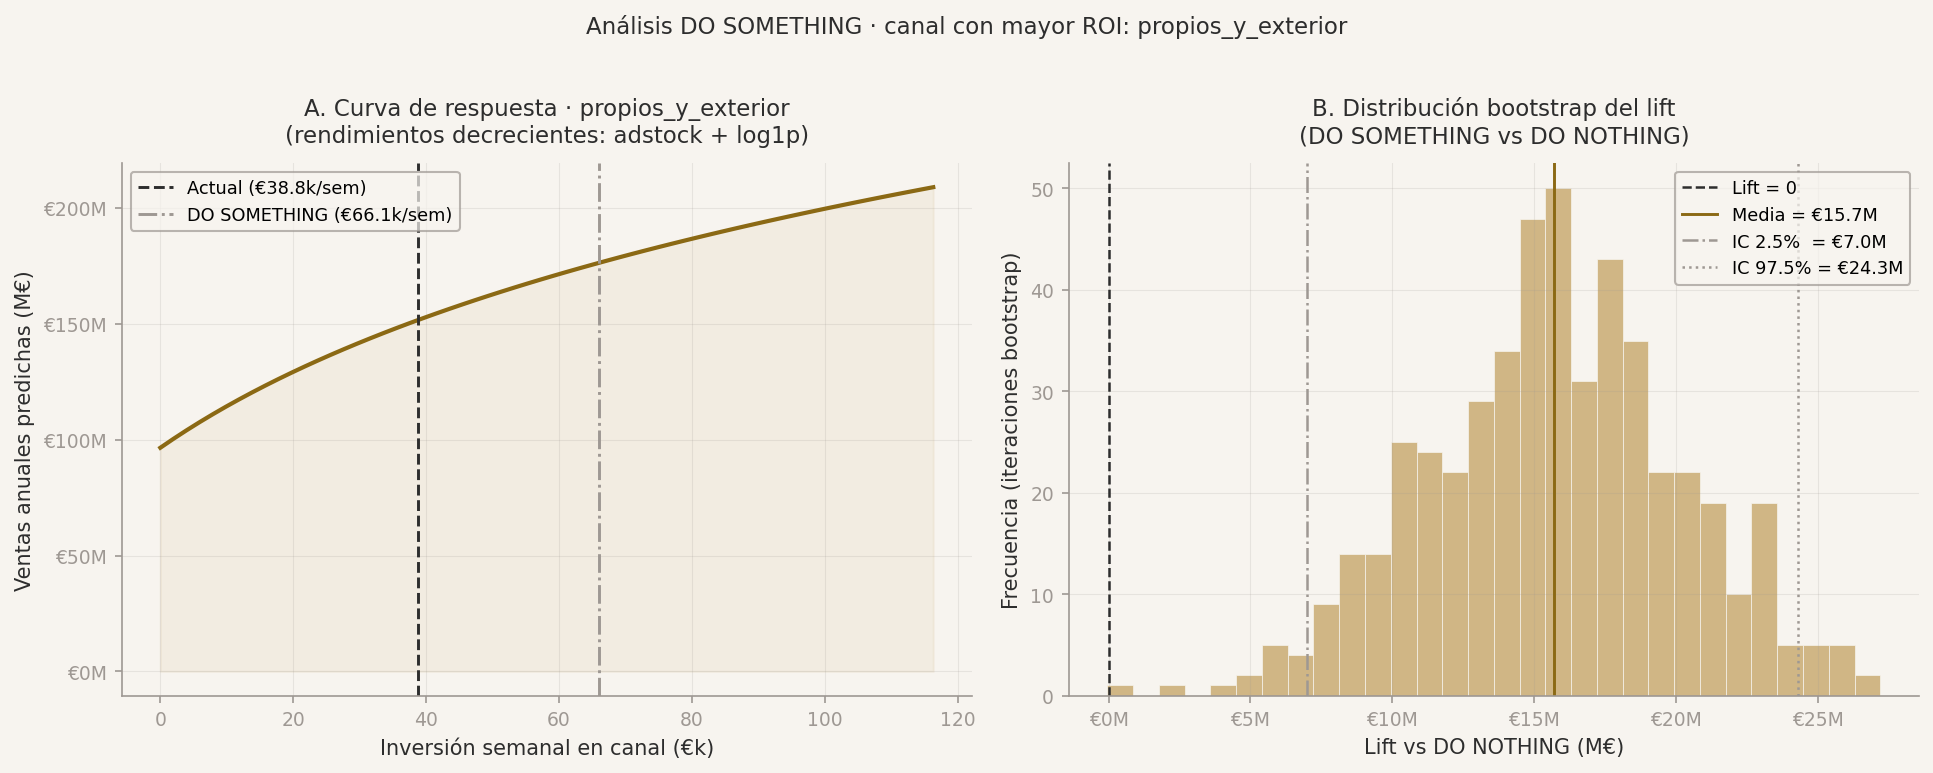
\includegraphics[width=\textwidth]{figures/ev_g5_curva_respuesta.png}
\caption{\textbf{Curvas de respuesta por grupo.} Muestran cómo reaccionan las ventas al aumentar la inversión en cada grupo, manteniendo los demás constantes. La zona continua es de crecimiento; la zona punteada es saturación (cada euro adicional rinde menos del 10\% del pico). Los puntos marcan el nivel histórico actual --- clave para identificar dónde hay recorrido y dónde no.}
\label{fig:ev_curva}
\end{figure}

\subsection{Presupuesto: baseline vs. propuesta}

\begin{figure}[htbp]
\centering
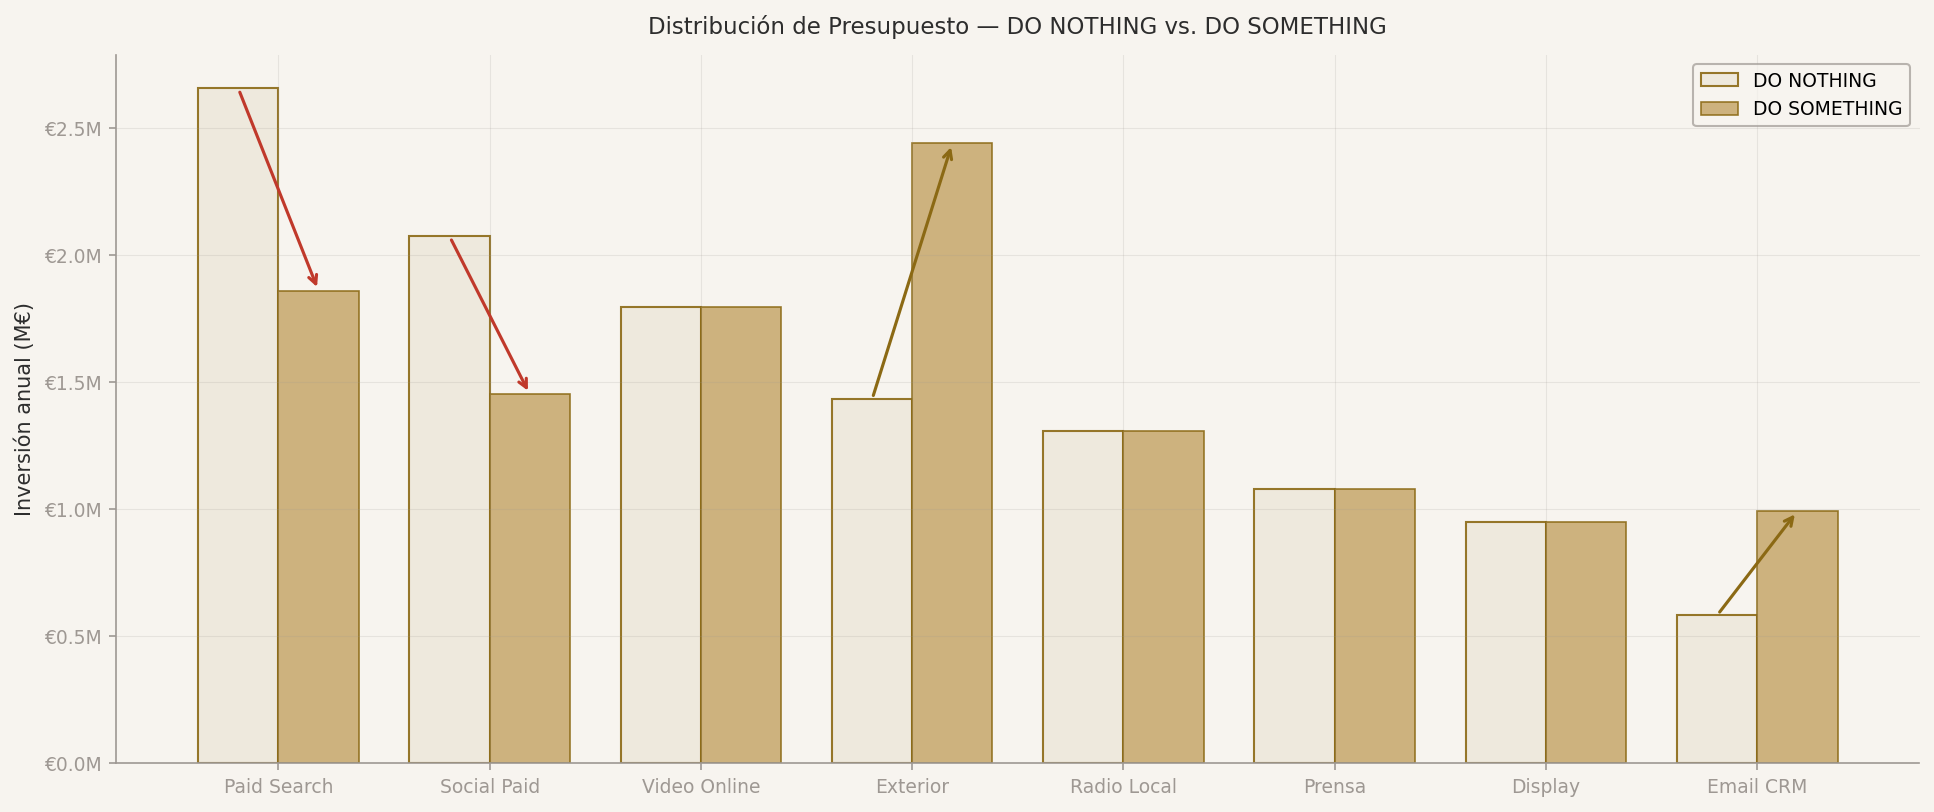
\includegraphics[width=\textwidth]{figures/ev_g6_presupuesto.png}
\caption{\textbf{Distribución del presupuesto: \textsc{Do Nothing} vs. \textsc{Do Something}.} Visualización grupo a grupo de la reasignación propuesta. El 30\% que sale de Performance entra en Propios y Exterior.}
\label{fig:ev_presupuesto}
\end{figure}

\begin{figure}[htbp]
\centering
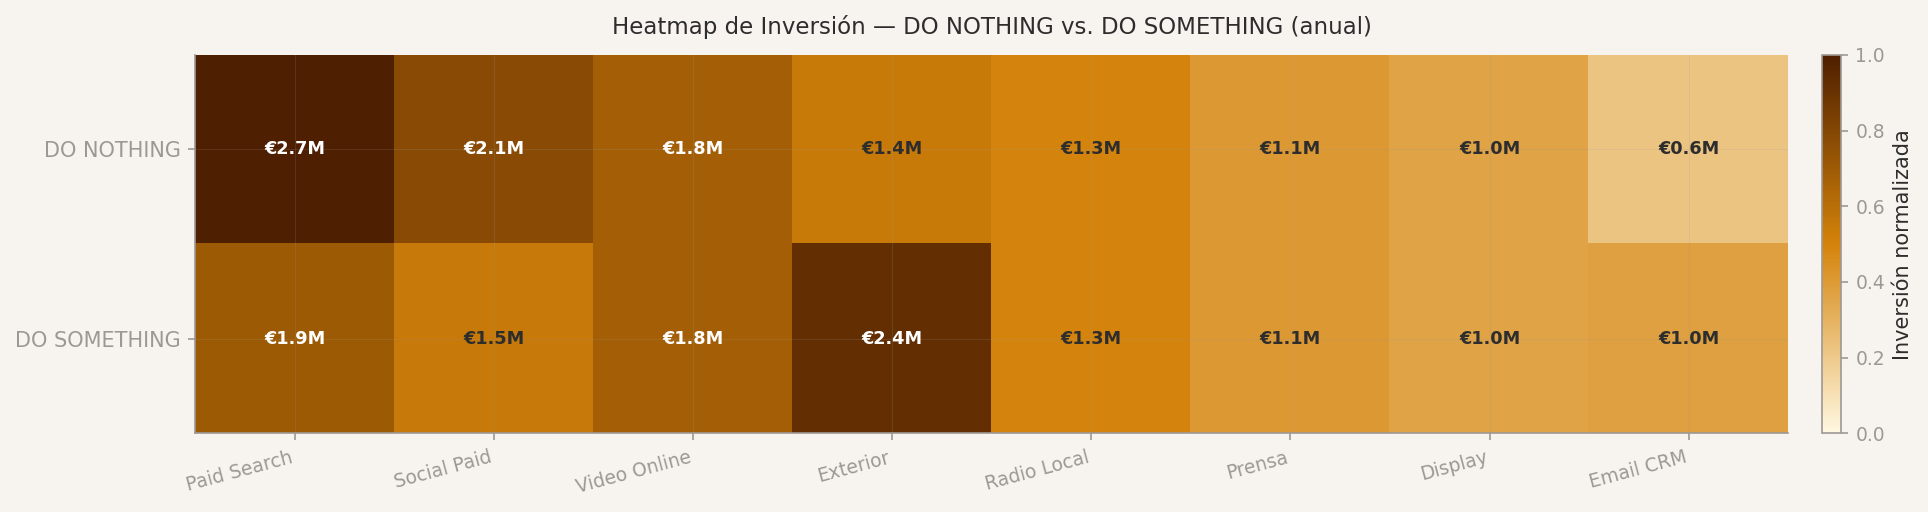
\includegraphics[width=\textwidth]{figures/ev_g8_heatmap_inversion.png}
\caption{\textbf{Heatmap de inversión normalizada.} Intensidad proporcional al gasto en cada grupo bajo cada escenario. Una forma compacta de ver el \textit{antes} y \textit{después} del reparto.}
\label{fig:ev_heatmap}
\end{figure}

\subsection{Tornado de sensibilidad}

\begin{figure}[htbp]
\centering
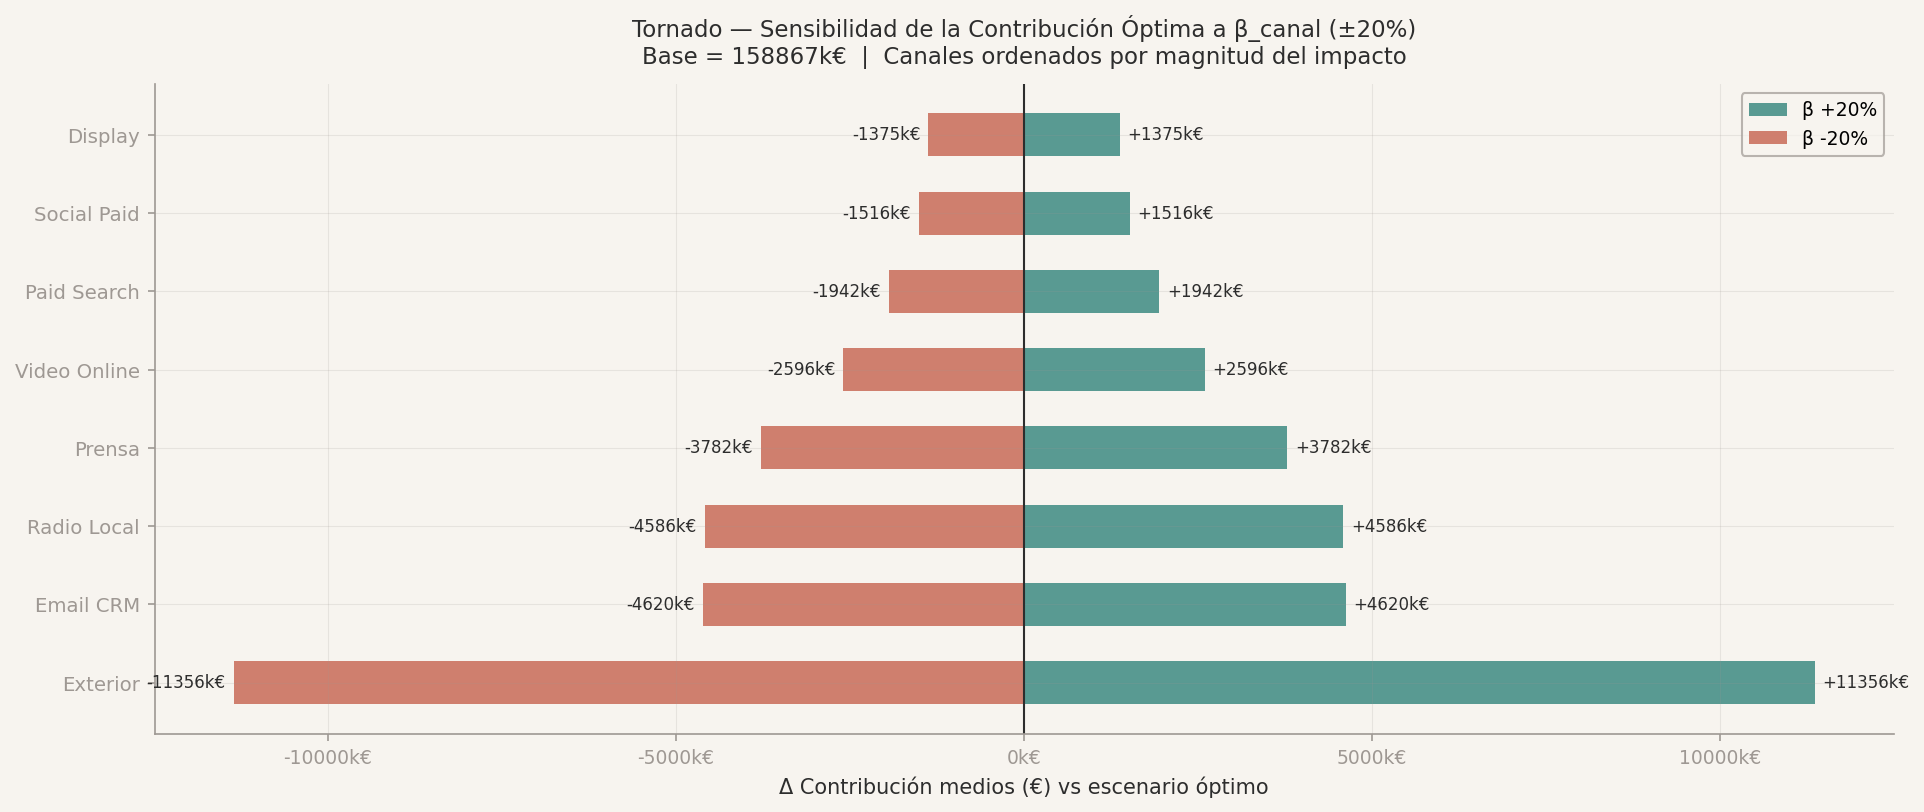
\includegraphics[width=\textwidth]{figures/ev_g7_tornado.png}
\caption{\textbf{Sensibilidad a $\pm 20\%$ en los $\beta$.} Muestra cuánto cambiaría la contribución total del marketing si el coeficiente de cada grupo fuera un 20\% mayor o menor. Los grupos con barras largas (\textit{Propios y Exterior} y \textit{Offline Medios}) son los que más influyen en el resultado — son los que más cuidado exigen al reasignar presupuesto.}
\label{fig:ev_tornado}
\end{figure}

\subsection{Lectura para comité}

\begin{takeaway}
\begin{enumerate}[leftmargin=*, itemsep=3pt]
    \item \textbf{Orden de eficiencia claro y robusto:} Propios y Exterior (25.7$\times$) $>$ Offline Medios (15.3$\times$) $>$ Branding Digital (8.5$\times$) $>$ Performance (6.0$\times$).
    \item \textbf{Performance es el grupo saturado}: recibe 40\% del presupuesto publicitario pero genera el ROI más bajo de los cuatro.
    \item \textbf{Propios y Exterior está infrainvertido}: genera el mayor retorno por euro y recibe el menor presupuesto absoluto (10\,M€ de 58.9\,M€ totales).
    \item \textbf{Reasignar antes de aumentar}: el lift de \textsc{Do Something} se obtiene \textbf{sin aumentar el gasto total}.
    \item \textbf{Riesgo acotado}: los IC 95\% no cruzan cero y el tornado muestra que errores del $\pm 20\%$ en $\beta$ no invierten la ordenación.
\end{enumerate}
\end{takeaway}
